
\textbf{introduce the notation here instead of in the appendix}
This project is part of improving the performance of technologies that meet the challenges of the law concerning the energy transition.
The innovative KEEP (Kite Electrical Energy Production) technology developed at ENSTA enables the production of electrical energy from a kite capturing wind energy.
The first numerical models of the system show an increase of about 50\% in the efficiency of this technology compared to already existing ones \alter{\url{https://www.sciencedirect.com/science/article/pii/S0960148118308206}}.
In the short and medium term, the onshore and ship application with a power production ranging from a few tens to hundreds of kW is targeted, extension to an offshore production power capacity at a MW scale with 1000 sqm kites is an objective.
To do this, following developments are required: the improvement of the mechanical model and the theoretical analysis of the complete dynamic system.
\begin{itemize}
    \item configuration variables alpha, thetal, phil, R, tau
    \item ahat, rhat, lhat
    \item geometrical parameters a, l
For better handling of the kite, we have \( \ell > 10 \) meters while the length of the arm \( a \) is fixed to two meters.
Thus, we have that
\begin{equation} \label{eq:ineq-l-a}
    \ell > a
\end{equation}
    \item other parameters
\end{itemize}


\section{Mathematical model of KEEP}
\subsection{Configuration manifold and kinematics}
The system, depicted in Fig.~\ref{fig:config}, consists of a rigid arm of length \(a\), rotating about the vertical axis at the origin \(O\), and a kite \(K\) connected to the tip \(A\) of the arm by lines of length \(\ell\).
We define a direct orthonormal reference frame \((O,\vu x,\vu y,\vu z)\), where \(\vu x\) and \(\vu z\) point respectively downwind and upward. The position of the arm tip is
\begin{equation}
    \vb a = \OA = \begin{pmatrix} a \cos\alpha \\ a \sin\alpha \\ 0 \end{pmatrix}
\end{equation}
where \(\alpha\in \in  \mathbb{S}^1\) is the angle of the arm relative
to the \(x\)-axis.
The motion of the kite is restricted to a conical surface centered at \(O\), generated by a lemniscate on the unit sphere. Its position
is expressed as
\begin{equation}
    \vb r = \OK = r\vu r(\tau),
\end{equation}
where \(r>0\) is the distance from the origin and
\begin{equation} \label{eq:sphere_Model_Deriv}
    \vu r(\tau) = \begin{pmatrix} \sin\theta(\tau)\cos\phi(\tau) \\ \sin\theta(\tau)\sin\phi(\tau) \\ \cos\theta(\tau) \end{pmatrix}.
\end{equation}
The lemniscate is parameterized by
\begin{equation} \label{eq:traject_Model_Deriv}
    \theta(\tau) = \theta_0 + \Delta\theta \sin(2\tau), \quad \phi(\tau) = \Delta\phi \sin(\tau),
\end{equation}

\begin{figure}
  \centering
  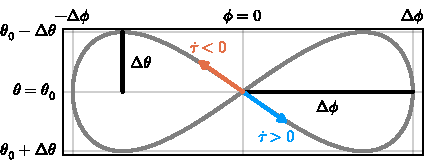
\includegraphics[width=0.6\textwidth]{figs/eight_plot}
  %\caption{The lemniscate that forms the base of the cone of constraints for the kite motion is parameterized by $\tau$ and its shape is controlled by design parameters $\theta_0$, $\Delta\theta$ and $\Delta \phi$. If $\tau$ increases (blue), the kite ascends in the middle and descends on the sides, while it is the opposite for a decreasing $\tau$ (orange). $\tau$ is increasing for a kite that ascends in the middle and descends on the sides (blue) while it is decreasing for the opposite (orange). The $y$-axis is flipped to reflect the orientation of the kite's trajectory.}
  \caption{The lemniscate, which forms the base of the kite's cone of constraints, is parameterized by $\tau$ and its shape is controlled by the design parameters $\theta_0$, $\Delta\theta$, and $\Delta\phi$. Trajectories with increasing $\tau$ (blue) result in a flight path that ascends in the middle and descends at the sides, while decreasing $\tau$ (orange) produces the inverse motion. The $y$-axis is inverted to align with the orientation of the kite's trajectory.}
  \label{fig:eight_plot}
\end{figure}

where \( \tau \in  \mathbb{S}^1 \), \( \theta_0 \) is the mean polar angle, and \( \Delta \theta \) and \( \Delta \phi \) are the amplitudes of the polar and azimuthal oscillations, respectively.

\begin{figure}
  \centering
  \includestandalone[width=0.6\textwidth]{figs/configuration}
  \caption{Configuration of the system. The vector $\mathbf{OA}$ represents the arm, connected at point $A$ (tip of the arm) to the kite $K$ by the lines $\mathbf{AK}$.}
  \label{fig:config}
\end{figure}

\begin{figure} 
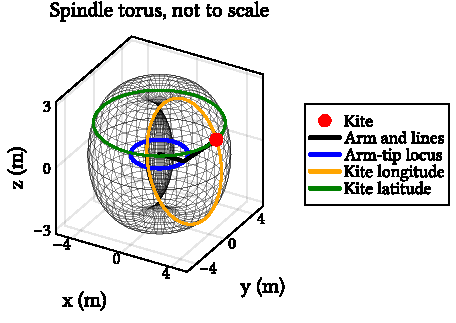
\includegraphics[width=0.6\textwidth]{figs/spindle_torus}

\alter{remove title, labels, tick labels, rescale properly ?}
\end{figure}

The fixed length of the lines imposes a geometric constraint. Defining \( \vb \ell = \AK \), we get
\begin{equation} \label{eq:loop}
    \boldsymbol{\ell} = \vb r - \vb a  \mathbf{\ell}  \text{\alter{ vb ell and ell result in the same glyph. use $\underline{\ell} ?$}}
\end{equation}
which, using \(\norm{\vb\ell}=\ell\), yields
\begin{equation}
    \ell^2 - r^2 + 2 r \vu r \vdot \vb a - a^2 = 0.
\end{equation}
Introducing the projection of the arm onto the radial direction, 
$$
p(\alpha, \tau) = \vu r \vdot \vb a = = a \sin\theta(\tau) \cos(\phi(\tau) - \alpha), $$
the constraint becomes
\begin{equation}
    r^2 - 2 p(\alpha, \tau) r + a^2 - \ell^2 = 0.
\end{equation}
Choosing the positive root corresponding to the kite above ground gives
\begin{equation}
    r(\alpha, \tau) = p(\alpha, \tau) + \sqrt{p(\alpha, \tau)^2 + \ell^2 - a^2}.
\end{equation}
Consequently, the position of the kite is entirely given by
\begin{equation}
    \vb r(\alpha, \tau) = r(\alpha, \tau) \vu r(\tau) 
\end{equation}
We therefore choose \(\vq=(\alpha,\tau)\) as generalized coordinates, which fully describe the configuration of the system.
The corresponding generalized velocities are
\(\dq=(\dot\alpha,\dot\tau)\). The velocity of the arm tip is
\begin{equation}
    \dot{\vb a} = \pdv{\vb a}{\vq} \dq
    = \begin{pmatrix} -a \sin \alpha & 0 \\ a \cos \alpha & 0 \\ 0 & 0 \end{pmatrix} \begin{pmatrix} \dot{\alpha} \\ \dot{\tau}  \end{pmatrix}
    = a \begin{pmatrix} -\sin \alpha \\ \cos \alpha \\ 0 \end{pmatrix} \dot \alpha,
\end{equation}
while the velocity of the kite is:
\begin{equation}
    \dot{\vb r} = \pdv{\vb r}{\vq} \dq
\end{equation}
The latter expression is kept in implicit form to streamline the flow of the discussion. Derivatives can be obtained for numerical implementation purposes via \ac{ad}.

\alter{clarify}

\alter{add definition of power and work. Copied from \textbf{section3-optimization.tex}
The average power is given by
\begin{equation}
    \bar P = W_f/t_f
\end{equation} where \(W_f\) is the total work done during one limit cycle and \(t_f\) is its period. We augment the state of our dynamical system with \(W\) that verifies:
\begin{equation}
\begin{cases}
    W(0) = 0 \\
    \dot W(t) = \dot W(t) = - \dot \alpha \, T(\dot \alpha) = b \, \dot \alpha^2 \quad (\geq 0),
\end{cases}
\end{equation}
}

% \begin{equation}
%     \dot{\vb r} = \pdv{\vb r}{\alpha} \dot{\alpha} + \pdv{\vb r}{\tau} \dot{\tau}.
% \end{equation}
% The partial derivatives of the radial distance \( r(\alpha, \tau) \) are given by:
% \begin{equation}
%     \pdv{r}{\alpha} = \pdv{p}{\alpha} \frac{r}{\sqrt{p^2 + \ell^2 - a^2}}, \quad \pdv{r}{\tau} = \pdv{p}{\tau} \frac{r}{\sqrt{p^2 + \ell^2 - a^2}}
% \end{equation}
% where the partial derivatives of \( p(\alpha, \tau) \) are:
% \begin{align}
%     \pdv{p}{\alpha} &= a \sin\theta(\tau) \sin(\phi(\tau) - \alpha) \\
%     \pdv{p}{\tau} &= a \theta'(\tau) \cos\theta(\tau) \cos(\phi(\tau) - \alpha) - a \phi'(\tau) \sin\theta(\tau) \sin(\phi(\tau) - \alpha)
% \end{align}
% with the derivatives of the spherical coordinates relative to the curve parameter \( \tau \) defined as:
% \begin{equation}
%     \theta'(\tau) = 2 \Delta\theta \cos(2\tau), \quad \phi'(\tau) = \Delta\phi \cos(\tau).
% \end{equation}
% The derivative of the unit radial vector \( \vu r(\tau) \) is:
% \begin{equation}
%     \dv{\vu r}{\tau} = \begin{pmatrix} 
%         \theta'(\tau)\cos\theta(\tau)\cos\phi(\tau) - \phi'(\tau)\sin\theta(\tau)\sin\phi(\tau) \\ 
%         \theta'(\tau)\cos\theta(\tau)\sin\phi(\tau) + \phi'(\tau)\sin\theta(\tau)\cos\phi(\tau) \\ 
%         -\theta'(\tau)\sin\theta(\tau) 
%     \end{pmatrix}.
% \end{equation}

\subsection{Force model}
%kite:
% - inertia
% - gravity
% - aero
% - line tension
% - fictitious cone force
%arm:
% - inertia
% - resistive torque
% - line torque

We model the wind velocity profile \( \vb w \) using a standard power-law wind shear model \addcite{1/7 power law}. Since the unit vector \( \vu x \) points downwind, the wind field is given by:
\begin{equation}
    \vb w(z) = w_{\text{ref}} \qty(\frac{z}{z_{\text{ref}}})^{1/7} \vu x
\end{equation}
where \( w_{\text{ref}} \) is the reference wind speed at altitude \( z_{\text{ref}} \). The altitude of the kite, $z$, is given by
\begin{equation}
    z = \vb r \vdot \vu z = r(\alpha, \tau) \cos\theta(\tau).
\end{equation}
The apparent wind velocity experienced by the kite is thus
\begin{equation}
    \vb w_a = \vb w(z) - \dot{\vb r}.
\end{equation}


The kite is subject to gravity, aerodynamic force, line tension, and the residual force constraining its prescribed conical motion. Gravity is modeled as
    \begin{equation} \label{eq:f_grav}
        \vb F_g = -\qty(m + \frac{m_\ell}{2}) g \vu z
    \end{equation}
where \(m_\ell = n \pi \ell \rho_\ell d_\ell^2 / 4\) is the total mass of the lines, half of which is assumed to be lifted by the kite.

The aerodynamic resultant is computed from the apparent wind using the same model detailed in Section~\ref{sec:model10D-dyn-aero}, namely:
    \begin{equation} \label{eq:f_aero}
        \vb F_a = L \vu k_t + D \vu k_b + \tilde D_\ell \vu k_b,
    \end{equation}
where the lift \(L\) and drag \(D\) are proportional to \(\norm{\vb w_a}^2\), and the line drag \(\tilde D_\ell\) is given by the integral approximation provided in Appendix~\ref{refappendix}.

The arm rotates about the axis \(\Delta = (O, \vu z)\) with moment of inertia \(I\).
It is subject to the torque exerted by the lines at $A$, and to the resistive torque of the generator, modeled as
\begin{equation}
    T(\dot\alpha)=-b\dot\alpha.
\end{equation}
The force exerted by the lines on the arm is \(-\vb F_\ell\), whose moment about \(\Delta\) is
\begin{equation} \label{eq:moment_fell}
        M_\Delta(-\vb F_\ell) = a F_\ell \lhat \vdot (\vu z \times \ahat).
\end{equation}
Newton's second law for the arm yields
\begin{equation} \label{eq:newton_arm}
    I \ddot\alpha = a F_\ell \lhat \vdot (\vu z \times \ahat) - T(\dot \alpha),
\end{equation}
    \alter{Error +T or \(T=b\dot{\alpha} \, with\, b>0\)}
from which the line tension is expressed as
    \begin{equation} \label{eq:f_lines}
        F_\ell = \frac{-I \ddot\alpha - T(\dot \alpha)}{a \lhat \vdot (\vu z \times \ahat)},
        \qquad
        \vb F_\ell = -F_\ell \lhat.
    \end{equation}

\subsection{Equations of motion}
The prescribed trajectory of the kite is enforced through a frictionless geometric constraint. The corresponding  eight-shaped coneical shape is
    \begin{equation}
        \mathcal{C} = \{\, R \rhat(\tau) \mid R>0,\ \tau\in[0,2\pi) \,\}.
    \end{equation}
Its tangent space is spanned by \(\partial\OK/\partial R = \rhat\) and \(\partial\OK/\partial\tau = R \rhat'\).
According to d'Alembert's principle, the constraint force, \(\vb F_c\), performs no virtual work along admissible displacements, so that:
    \begin{equation} \label{eq:cone_constraint}
        \vb F_c \vdot \rhat = 0,\qquad
        \vb F_c \vdot \rhat' = 0.
    \end{equation}
Newton's second law for the kite reads
    \begin{equation} \label{eq:newton_kite}
        m \ddot{\vb r} = \vb F_a + \vb F_g + \vb F_\ell + \vb F_c.
    \end{equation}
Combining this equation with the arm's dynamics and eliminating the constraint force using \eqref{eq:cone_constraint} yields a \(2\times2\) linear system for the generalized accelerations:
    \begin{equation} \label{eq:eom_implicit}
        M(\vq) \ddq = \vb h(\vq, \dq),
    \end{equation}
    whose explicit solution is derived in Section~\ref{sec:explicit-ddq} \alter{keep that annex?}.

\alter{Lonely sentence} We write the state of the dynamical system \(vb x = (\vq, \dq) = (\alpha, \tau, \dot \alpha, \dot \tau\) and define the evolution function \(f\) as
\begin{equation}
    f(\vb x) = f(\vq, \dq) = (\dq, \ddq),
\end{equation}
where \(\ddq\) is solution to \ref{eq:eom_implicit}.
The system is symmetric through the map
\begin{equation}
\label{eq:symmetry}
    \sigma: (\alpha, \tau, \dot \alpha, \dot \tau) \mapsto (-\alpha, \tau + \pi, -\dot \alpha, \dot \tau)
\end{equation}

The mechanical power extracted by the generator is
\begin{equation}
    \dot W(t)
    = -\dot\alpha\,T(\dot\alpha)
    = b\dot\alpha^2\geq0,
\end{equation}
where \(W(0)=0\). The average power of a solution spanning \([0, t_f]\) is
\begin{equation}
    \bar P=\frac{W_f}{t_f},
\end{equation}
where \(W_f=W(t_f)\) is the total extracted work.










% We apply Newton's second law of motion to the kite :
% \begin{equation}
%     \sum \vb F_i = m \dot{\vb r}
% \end{equation}

% All force formulas derived in \ref{sec:model10D-dynamics} still apply here, except for \ref{eq:newton_arm} because \( \theta \) and \( \phi \) are not defined anymore.
% % Why ?
% % The relationship between the line tension at \( A \) — \( -\vb F_\ell = - F_\ell \lhat \), and the moment it applies on the arm around axis \( \Delta = (O, \vu z) \) passing through \( O \) with direction \( \vu z \) — \( M_\Delta(-\vb F_\ell) \), 
% Instead of computing these angles from the \( q \), we derive a new formula:
% \begin{equation}
%     M_\Delta(\vb F_\ell) = a F_\ell \lhat \vdot (\vu z \times \ahat)
% \end{equation}

% \begin{proof}
% The lines apply of force \( -\vb F_\ell \) on the arm \( \OA \) at point \( A \), which rotates around \( \Delta \).
% The corresponding moment is
% \begin{equation}\begin{split}
%     M_\Delta(-\vb F_\ell) &= \vb M_O(-\vb F_\ell) \vdot \vu z = [\OA, -\vb F_\ell, \vu z] = [a \ahat, F_\ell \lhat, \vu z] = a F_\ell [\lhat, \vu z, \ahat] \\
%     &= a F_\ell \lhat \vdot (\vu z \times \ahat),
% \end{split}
% \end{equation}
% where \( [\vb a, \vb b, \vb c] = (\vb a \times \vb b) \vdot \vb c \) denotes the triple product, which is invariant under circular shift, and \( \vu z \times \ahat \) is simply \( (-\sin(\alpha), \cos(\alpha), 0) \).


% \alter{<remove label="circular shift proof">}
% We write \( \lhat \) in the base attached to the arm \( (\ahat, \vu z \times \ahat, \vu z) \):
% \begin{equation}
%     \lhat = (\lhat \vdot \ahat) \ahat + (\lhat \vdot (\vu z \times \ahat)) (\vu z \times \ahat) + (\lhat \vdot \vu z) \vu z
% \end{equation}
% to easily develop the triple product into
% \begin{equation}
%     M_\Delta(\vb F_\ell) = (a \ahat \times F_\ell \lhat) \vdot \vu z = a F_\ell \lhat \vdot (\vu z \times \ahat).
% \end{equation}
% \alter{</remove>}
% \end{proof}

% \subsection{Newton's second law}
% The arm has inertia \( I \) and the electrical generator applies torque \( T : \omega \mapsto -b \omega \) where b is analogous to a rotational viscous damping coefficient, with dimension of torque per angular velocity.
% Applying Newton's second law to the arm gives
% \begin{equation}
%     I \ddot \alpha = M_\Delta(\vb F_\ell) + T(\dot \alpha) = \alpha F_\ell \lhat \vdot (\vu z \times \ahat) - b \dot \alpha,
% \end{equation}
% from which we obtain \( \vb F_\ell \), pointing from the \( K \) to \( A \), thus in the direction of \( -\lhat \):
% \begin{equation} \label{eq:f_lines}
%     \vb F_\ell = \frac{-I \ddot \alpha - b \dot \alpha}{a \lhat \vdot (\vu z \times \ahat)} \lhat
% \end{equation}

% \alter{put this at the right place}
% The wind profile is parameterized by \( z_0 \), a reference altitude, and \( w_0 \), its speed at this altitude.
% Using the 1/7th power rule \alter{\url{https://journals.ametsoc.org/view/journals/apme/17/3/1520-0450_1978_017_0390_otuopl_2_0_co_2.pdf}}, we obtain
% \begin{equation}
%     \vu w(z) = w_0 (\frac{z}{z_0})^\frac{1}{7} \vu x.
% \end{equation}


% The forces applied to the kite are:
% \begin{itemize}
%     \item gravity \( \vb F_g = -(m + m_\ell/2) g \vu z \)
%     \item aerodynamic resultant \( \vb F_a = L \vu k_t + (D + \tilde D_\ell) \vu k_b \), the detailed computation is found in \ref{sec:model10D-dyn-aero}
%     \item line tension \( \vb F_\ell \) computed in \ref{eq:f_lines}
%     \item the fictitious cone force \( \vb F_c \) that still needs to be determined.
% \end{itemize}

% We apply Newton's second law to the kite and isolate \( \vb F_c \)
% \begin{equation} \label{eq:f_cone_newton}
%     \vb F_c(\vq, \dq, \ddq) = m \ddot \OK(\vq, \dq, \ddq) - \vb F_g - \vb F_a(\vq, \dq) - \vb F_\ell(\vq, \dq, \ddq).
% \end{equation}
% For the kite to stay on the eight-shaped cone, we choose \( \vb F_c \) to be the solution of
% \begin{equation}\begin{cases} \label{eq:f_cone_constraint}
%     \vb F_c \vdot \pdv{\OK}{R} = 0 \\
%     \vb F_c \vdot \pdv{\OK}{\tau} = 0
% \end{cases}\end{equation}
% \alter{use \( \tilde \OK(R, \tau) \) instead of \( \OK(\alpha, \tau) \) ? Should I even keep \( \tilde \OK \) ? It's more mechanics than maths}
% so that the kite glides without friction on the cone.
% Given some generalized coordinates \( \vq \) and velocities \( \dq \), this system of \( 2 \) equations can be solved for the accelerations \( \ddq \in \R^2 \), therefore defining a second order \ac{ode} on \( \vq \).

% Let's compare this result to that of \ref{sec:model10D}.
% We had a \ac{dae} of dimension \( 5 \) with \( 2 \) \ac{dof} and \( 3 \) constraints, while by computing essentially the same quantities but only using generalized coordinates \( \vq = (\alpha, \tau) \), we have an easier problem to solve with fewer calculations.
% We go a step further by solving this system without a symbolic solver, thus writing \( \ddq \) explicitly in terms of \( \vq \) and \( \dq \); see \ref{sec:explicit-ddq} for the detailed calculation.
% The result is
% \begin{equation}
%     2
% \end{equation}